\chapter{Propiedades macroscópicas y de estructura}

En este capítulo se describen las ecuaciones y los métodos usados para extraer resultados del sistema de este trabajo, como la función de distribución radial, la temperatura, energía y presión. Al final de este capítulo se detalla el sistema simulado.

\section{Función de distribución radial y el número de coordinación}
% \textcolor{red}{usar mejor la definición de VMD para enlazar bien el marco teórico con la metodología}

Esta función es importante ya que el objetivo de esta es la extracción de información estructural del sistema en todos los cuadros (tiempo) de simulación, como se vio en el capitulo \ref{chap:mecanica_estadistica} gracias a la hipótesis ergódica, estas mediciones son iguales a medirlo en el tiempo como en este trabajo a como sería medirlo en el ensamble como corresponde en el caso experimental de un ensamble NPT del mismo sistema.\\

La función de distribución radial representa la probabilidad de encontrar un átomo en una cascara $dr$ a una distancia $r$ de otro átomo elegido como punto de referencia como en la figura \ref{fig:gr}. En la dinámica molecular, la función de distribución radial es como se muestra en la ecuación (\ref{gr}) \cite{LEVINE20113556}.\\

\begin{equation} \label{gr}
    g(r)=\lim_{dr\to 0} \frac{p(r)}{4\pi \left(N_{pares}/V\right)r^{2}dr}
\end{equation}\\

donde $r$ es la distancia entre átomos, $p(r)$ es el promedio del número de pares de átomos encontrados a una distancia $r$ y $r+dr$, V el volumen total del sistema y $N_{pares}$ es el número de pares únicos de átomos donde un átomo es de cada uno de dos conjuntos, $sel_1$ y $sel_2$.\\

\begin{figure}[!h]
    \centering
    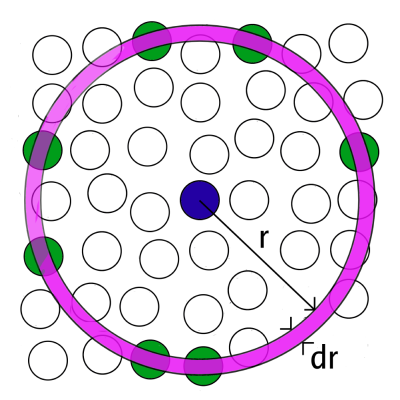
\includegraphics[width=.2\textwidth,keepaspectratio=true]{gr.png}
    \caption{Evaluación de la función de distribución radial}
    \label{fig:gr}
\end{figure}

El promedio $p(r)$ es calculado sobre toda la trayectoria de una simulación con $N_{cuadros}$ el número total de cuadros en la simulación. Este promedio toma la forma de:\\

\begin{equation}\label{p}
    p(r)=\frac{1}{N_{cuadros}}\sum^{N_{cuadros}}_i \sum_{j\in sel1} \sum_{k\in sel2} \sum_{\kappa} d_{\kappa}(r_{ijk})
\end{equation}\\

donde $\kappa$ son los índices de los contenedores del histograma y

\begin{equation}
    d_{\kappa}(r_{ijk}) = 
    \begin{cases}
        1 / \Delta r &\text{si $r_\kappa \leqq r<r_\kappa + \Delta r$ y $r_\kappa \leqq r_{ijk}<r_\kappa + \Delta r$}\\
        0 & \text{de otra manera}\\
    \end{cases}
\end{equation}

donde $\Delta r$ es el ancho de los contenedores del histograma y $r_\kappa$ es la distancia mínima asociada con cada contenedor, dado por:

\begin{equation}
    r_\kappa = r_0 + \kappa \Delta r
\end{equation}

con $r_0$ el límite inferior del histograma.\\

El cálculo de la función de distribución radial también cumple con la convención de mínima imagen. El límite superior del histograma debería no ser mayor a $L/2$.\\

La integración de la función de distribución radial genera el número de coordinación $n(r)$, el cual es un recuento del número de vecinos a una distancia radial determinada \cite{GOCHENOUR201841}. para el caso de la simulación, es el promedio en todos los cuadros.\\

\section{Propiedades macroscópicas del sistema}

\subsection{Energía}

El promedio de la energía es trivialmente calculada como el promedio de la ecuación (\ref{hamiltoniano}) \cite{Allen2017}:

\begin{equation} \label{promenergia}
    \langle E \rangle = \left \langle\sum_{i=1}^{N} \frac{1}{2 m_i}\dot{\vec{p_i}}^2 \right \rangle+ \left \langle\sum_{i=1}^{N-1}\sum_{j=i+1}^{N} u(r_{ij})\right \rangle
\end{equation}

\subsection{Temperatura}

Por el teorema del virial tenemos la siguiente ecuación \cite{Allen2017}:

\begin{equation} \label{virialtheorem}
    \left \langle p_k \frac{\partial H}{\partial p_k} \right \rangle = k_B T
\end{equation}

Para el hamiltoniano en la ecuación (\ref{hamiltoniano}) encontramos:

\begin{equation} \label{virialtemp}
    K_B T = \left \langle p_k \frac{p_k}{m_k} \right \rangle
\end{equation}

entonces derivamos la siguiente ecuación al incorporar la suma para los 3N términos de N partículas:

\begin{equation} \label{virialsumtemp}
    3NK_B T = \left \langle \sum_{k=1}^{N}\frac{|p_k|^2}{m_k} \right \rangle
\end{equation}

Para un sistema simulado donde hay $N_C$ restricciones de algún tipo (e.g. descripciones de centro de masa, ángulos rígidos, enlaces rígidos entre otros), la ecuación anterior se convierte en:

\begin{equation} \label{virialsumconsttemp}
    T= \frac{1}{3(N - N_C)K_B}\left \langle \sum_{k=1}^{N}\frac{|p_k|^2}{m_k} \right \rangle
\end{equation}

\subsection{Presión}

La otra ecuación del teorema del virial nos da la siguiente ecuación:

\begin{equation} \label{virialtheoremq}
    \left \langle q_k \frac{\partial H}{\partial q_k} \right \rangle = K_B T
\end{equation}

lo cual nos lleva a:

\begin{equation} \label{virialtheorempress}
    \frac{1}{3}\left \langle \sum_{i=1}^N \mathbf{r_i} \cdot f^{tot}_i \right \rangle = -N K_B T
\end{equation}

si dividimos la fuerza total entre externa e intermolecular llegamos a otra ecuación \cite{Allen2017}:

\begin{equation} \label{virialsumconstpress}
    P = \frac{N}{\left \langle V \right \rangle} K_B T + \frac{\left \langle \mathcal{W} \right \rangle}{\left \langle V \right \rangle}
\end{equation}

\begin{equation*}
     \text{donde } \mathcal{W} = \frac{1}{3} \sum_{i=1}^N \mathbf{r_i} \cdot f_i \text{ con $f_i$ fuerzas intermoleculares dado por el campo de fuerzas}
\end{equation*}

\section{Sistema simulado}

El sistema se simuló en un rango de temperaturas de 280 K a 370 K, este consta de 16807 moléculas de agua, 10 moléculas de ácido 2,4-diclorofenoxiacético (2,4-D) y un nanotubo de carbono (6, 5) de alrededor de 38 nm de largo. En todas las simulaciones se usó el termostato de nosé-hoover acoplado con un barostato parrinello-rahman con $\tau_t$ de 0.4 ps y $\tau_p$ de 1.6 ps respectivamente.\\

Todas las simulaciones constaron de 20 ns de tiempo de simulación, se usó algoritmo de salto de rana y radio de corte de 1.2 nm. La validez de los parámetros del termostato y barostato fue verificada revisando que las condiciones de simulación fueron mantenidas de manera adecuada conforme los valores impuestos en la simulación NPT, como se muestra en la tabla \ref{tab:promediostemppres}.

\begin{table}[h!]
    \centering
    \begin{tabular}{ |m{6em}|m{5em}||m{5em}|m{5em}|  }
    \hline
    Temperatura (K) & Error & Presión (bar) & Error \\
    \hline
    \hline
    280.003 & 0.0018 & 0.840079 & 0.12 \\
    298.149 & 0.0014 & 1.11589 & 0.099 \\
    309.998 & 0.0013 & 1.28056 & 0.2 \\
    319.996 & 0.0012 & 1.01285 & 0.12 \\
    329.998 & 0.0016 & 1.12986 & 0.079 \\
    340 & 0.0019 & 1.11812 & 0.13 \\
    349.998 & 0.0028 & 1.30148 & 0.13 \\
    360.003 & 0.0022 & 1.02411 & 0.13 \\
    370.002 & 0.002 & 1.1182 & 0.13 \\
    \hline
    \end{tabular}
    \caption{Promedio de temperatura y presión de los sistemas simulados.}
    \label{tab:promediostemppres}
\end{table}

% y el campo de fuerzas usado en el sistema es GROMOS 54A7, que tiene la siguiente forma en nuestras simulaciones:
% \begin{itemize}
%     \item Número de moléculas: 16807 moléculas de agua, 10 moléculas de ácido 2,4-diclorofenoxiacético (2,4-D) y un nanotubo de carbono (6, 5) con 364 átomos.
%     \item Integrador de todos los sistemas: salto de rana para las ecuaciones de movimiento de Newton.
%     \item Paso de tiempo: 0.002 ps, número de pasos: 10000000, Intervalo de tiempo: 20 ns.
%     \item radio de corte para la lista de vecinos de corto alcance: 1.2 nm, radio de corte para interacción de coulomb: 1.2 nm, radio de corte para interacción LJ 12-6: 1.2 nm.
%     \item Corrección de dispersión de largo alcance para energía y presión.
%     \item Acoplamiento de temperatura: ensamble extendido de nose-hoover con $\tau_t$: 0.4 ps y con las temperaturas antes mencionadas.
%     \item Acoplamiento de presión: ensamble extendido de parrinello-rahman con $\tau_p$: 1.6 ps a presión: 1 bar.
%     \item Algoritmo de constricción: LINCS(LINear Constraint Solver).
% \end{itemize}




